
\documentclass[a4paper,alpha-refs]{RBCA_v1.0}

\usepackage[portuguese=nohyphenation,english=nohyphenation]{hyphsubst}
% below is defined the main language of the paper - for paper in portuguese you must change "english" by "portuguese".
\usepackage[english]{babel} 
\usepackage{graphicx}
%%% Place your packages here
%%% \usepackage[options]{package}

%%%


%%% title of the paper
\title{A aplicação da derivada na detecção de bordas para alunos do primeiro período de engenharia}

%%% Use the \authfn to add symbols for additional footnotes, if any. 1 is reserved for correspondence emails; then continuing with 2 etc for contributions.
\author[1]{First Author}
\author[2]{Second Author}
\author[2]{Third Author}
\author[2]{Fourth Author}

\affil[1]{First Institution}
\affil[2]{Second Institution}

%%% Author e-mails
\authnote{\authfn{1}first@uni.edu; second@lab.edu; $\cdots$}

%%% "Short" author for running page header
\runningauthor{First et al.}

%%% Paper category:
%%% if in English  : Original paper,  Experience Report     or Tutorial
%%% if in Português: Artigo original, Relato de experiência ou Tutorial
\papercat{Original Paper}

%%% Information about the journal edition and the paper
%%% should only be set by editor
\jvolume{10}           % volume number
\jissue{1}             % issue number
\jyear{2018}           % edition year
\jmonth{April}         % edition month

\setcounter{page}{1}   % number of the first page of the paper
\jpages{1--4}          % paper page numbers
\jid{9999}             % paper ID 

\jrec{yyyy-mm-dd}      % date of article submission
\jrev{yyyy-mm-dd}      % date of final paper revision
\jacc{yyyy-mm-dd}      % date of paper accepted


\begin{document}

\begin{frontmatter}
	
\maketitle

\begin{Abstract} % abstract in english
The Abstract (250 words maximum) should be structured to include the following details: \textbf{Background}, the context and purpose of the study; \textbf{Results}, the main findings; \textbf{Conclusions}, brief summary and potential implications. Please minimize the use of abbreviations and do not cite references in the abstract.
\end{Abstract}

\begin{keywords}
Keyword1; keyword 2; keyword 3 (Three to five keywords representing the main content of the article, in alphabetic order)
\end{keywords}

\begin{resumo} % resumo em português
	O Resumo (com até 250 palavras) deverá ser estruturado para abordar os seguintes detalhes: \textbf{Background}, o contexto e propósito do estudo; \textbf{Resultados}, os principais encontrados; \textbf{Conclusões}, um breve resumo do trabaho e as implicações em potencial. Por favor, evite, na medida do possível, o uso de abreviaturas e não cite referências no resumo.
\end{resumo}

\begin{palavras_chave} % palavras-chave em português 
	Palavra-chave 1; palavra-chave 2; palavra-chave 3 (De três a cinco palavras-chave que representem os principais tópicos do artigo, em ordem alfabética)
\end{palavras_chave}

\end{frontmatter}


\section{Introduction to this Template}

The Revista Brasileira de Computação Aplicada (RBCA) is a \textbf{open access journal} linked to the \href{http://ppgca.upf.br}{Graduate Program in Applied Computing (PPGCA)} of the \href{http://www.upf.br}{University of Passo Fundo}, Brazil. RBCA aims to provide to the scientific community article that present an interdisciplinary perspective of the application of Computing in different areas of knowledge.

This is the \LaTeX{} template for RBCA journal manuscript submissions. \textcolor{red}{Submissions that do not use the format available in this template will be automatically rejected.} 

\textbf{Articles submitted to RBCA should be between 8 and 15 pages and will be published electronically.} The languages accepted by RBCA are Portuguese and English. We alert the authors that the preparation of the manuscript should be made carefully, both in its scientific content and in its grammatical correctness.

There are important commands in the preamble that you will need to modify for your own manuscript. Specify your manuscript's category with the \verb|\papercat{...}| command in the preamble. See the sample code in the preamble for a sample of how author, affiliation and e-mail information can be specified. Information about this edition of RBCA and publication details of the manuscript will be filled out by the journal's editor.

This template has been edited and validated in the \href{http://www.texstudio.org/}{TexStudio\copyright} program and the \href{https://www.overleaf.com/}{Overleaf\copyright} Collaborative Writing and Publishing System. Any questions or problems regarding this template should be reported to the e-mail of the journal (\textcolor{blue}{rbca@upf.br}).

The remainder of this current section will provide some sample \LaTeX{} code for various elements you may want to include in your manuscript.

\section{Processamento de imagem}

O processamento de imagem atua na separação de pontos de interesse por meio de operações que resultaram em uma imagem de saída. Utilizando imagens é possível extrair informações sobre as características físicas e geométricas básicas dos objetos, tais como a dimensão, a área, o perímetro e a forma.
 
Segundo \cite{ProcDigital} uma imagem pode ser representada como uma função bidimensional denotada por $f$(x,y), tal que x e y são coordenadas de um plano e $f$ expressa a intensidade de cinza nas coordenas. Existe um número finito de elementos no contra domínio dessa função e cada um é denominados como \textit{Picture element} (\textit{pixel}).


Para que um sistemas computacional reconheça os elementos de uma imagem é necessário a digitalização de cada pixel. Para isso são necessários dois procedimentos, primeiramente a amostragem e então a quantização. A amostragem consiste na seleção de pontos igualmente espaçados de uma função continua, que representa uma imagem, de forma que esses pontos sejam coletados gerando um conjunto de localizações discreta. Por outro lado, a quantização transforma os valores contínuos da intensidade de cores uma determinada amostra em valores discretos. Esses procedimentos possibilitam a alocação dos valores quantizados em uma matriz nas posições advindas do processo de amostragem. 

O armazenamento em uma matriz tem como vantagem a possibilidade da aplicação de operações matriciais sobre a fotografia. Nesse caso, os pixels são representados por uma coordenada (x, y) referente à sua posição no plano, e z, a intensidade da cor. Na área de computação visual adotou-se que a intensidade do pixel igual a 0 representaria o preto e o 255 representaria o branco, todas as outras cores são variações nesse intervalo. 

\begin{figure}[h!]
	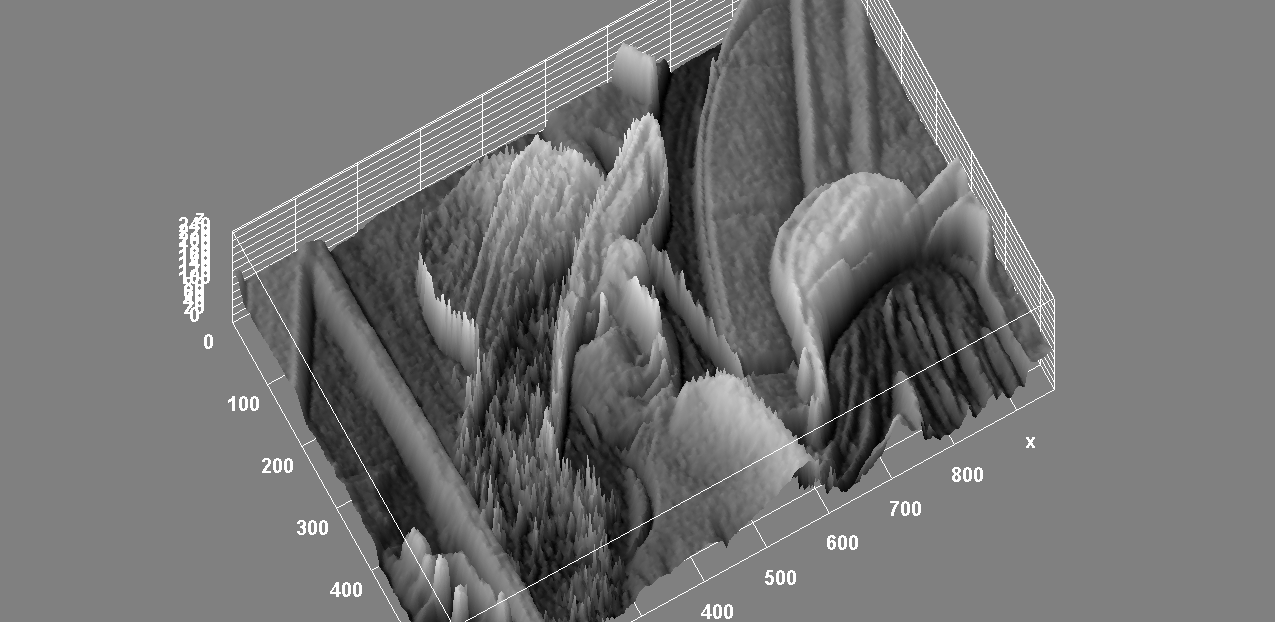
\includegraphics[width=.5\textwidth]{img/img1.png}
	\caption{Representação das dimensões da imagem e a intensidade de cada pixel}
	\label{img:lena3d}
\end{figure}

As imagens são, normalmente, representadas no sistema RGB (do inglês Red, Green and Blue), isso significa que cada pixel é uma aproximação resultante das intensidades de vermelho, azul e verde. A união das três cores em cada pixel forma uma imagem de 3 bandas \citep{biasi2002desenvolvimento}. Segundo \cite{de2006introduccao} a demonstração da imagem de três bandas pode ser a seguinte equação, tal que $F_r$, $F_g$ e $F_b$ representam respectivamente a intensidade das bandas vermelha, verde e azul:

\begin{equation}
F(x,y)=F_r(x,y)+F_g(x,y)+F_b(x,y)
\end{equation}

A par desses conceitos, o processamento se inicia transformando a imagem formada pelas bandas RGB em tons de cinza. Isso porque as variações entre as bandas serão analisadas apenas como uma variação de cinza. Segundo a documentação oficial dos desenvolvedores da biblioteca Opencv, incluída no algoritmo, a transformação aplicada é baseada em uma média ponderada das componentes RGB de cada pixel, dada pela fórmula a seguir:

\begin{equation}
F(x,y)=(0,299*F_r(x,y))+(0,587*F_g(x,y))+(0,114*F_b(x,y))
\end{equation} 


\begin{figure}[h!]
	\centering
	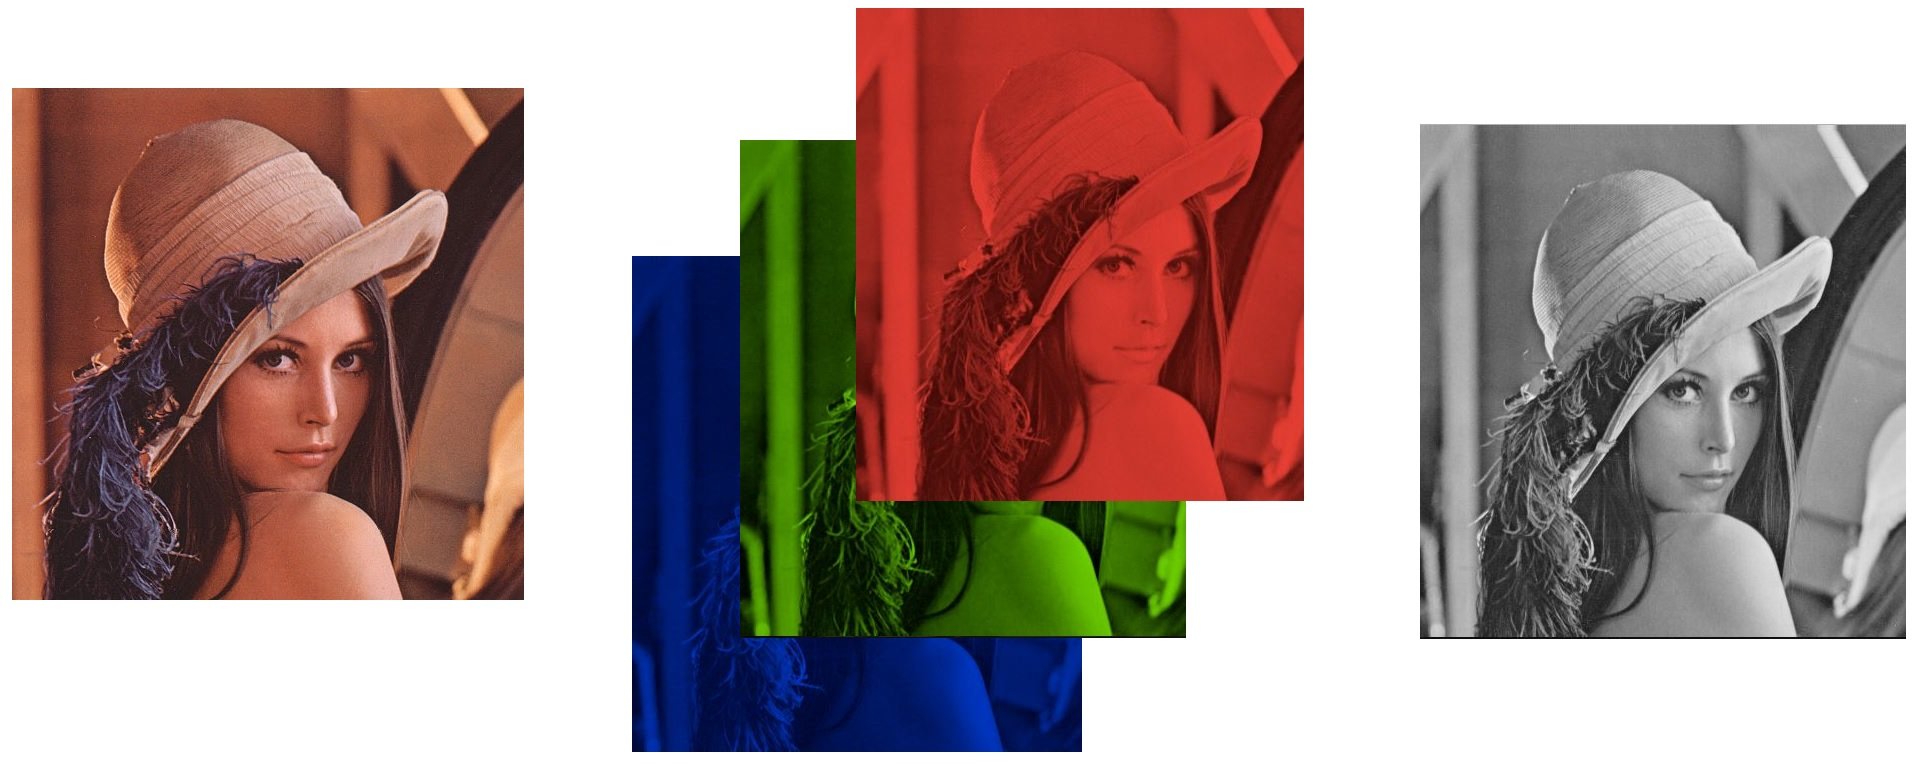
\includegraphics[width=.5\textwidth]{img/lenna_rgb_gray.jpg}
	\caption{Representação de uma imagem nas bandas RGB e em escala de cinza}
	\label{img:lenargb}
\end{figure}

Segundo \cite{de2006introduccao} existem duas classificações importantes quando se trata de operações que manipulam de forma direta o pixel: as operações pontuais e as operações locais ou por máscaras. Nas operações pontuais cada pixel é tratado de forma independente. Já nas operações locais ou por máscara o valor de saída depende de um conjunto de pixels vizinhos. É importante salientar, que as mascaras são matrizes com dimensões pequenas em que, o pixel a ser tratado é posicionado no centro da matriz de operação e o resultado é um novo valor na mesma posição.

A par desses conceitos é possível, então, aplicar o método para a detecção de borda desenvolvido por John Canny. A imagem de saída resultante da aplicação desse método é do tipo imagem binária, pois os elementos variam entre 0 ou 1, de forma que 1 representa que naquele pixel há uma borda.

\begin{figure}[h!]
	\centering
	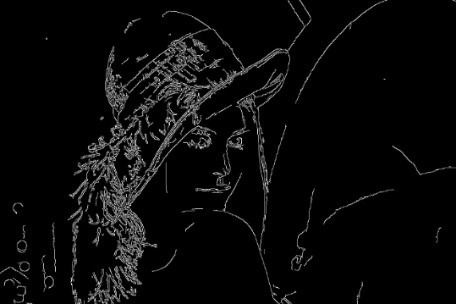
\includegraphics[width=.3\textwidth]{img/img9.jpg}
	\caption{Representação da borda de uma imagem}
	\label{img:lenaborda}
	
\end{figure}
\section{Métodos Canny para detecção de bordas}
\subsection{Suavização Gaussian}
\subsection{Detecção do gradiente}

Após a suavização de ruídos na imagem, os métodos de detecção das bordas precisam de ferramentas que proporcionem encontrar a localização de variações bruscas das cores. É nesse momento que os conceitos de derivadas são utilizados, por meio do gradiente.

O gradiente é um vetor bidimensional, denotado por $\nabla f$ , que representa a taxa de variação da função $f$ na posição (x,y) \cite[p. 465]{ProcDigital}. É necessário utilizar esse tipo de ferramenta uma vez que, como foi visto, a imagem pode ser vista como uma função de duas dimensões, podendo ocorrer variações de intensidade cores tanto em relação ao eixo x quanto ao eixo y. 

\begin{equation}
\nabla f = (Gx,Gy) = (\frac{\partial f}{\partial x},\frac{\partial f}{\partial y})
\label{eq:gradiente}
\end{equation}

No contexto do processamento de imagem, o gradiente fornecerá a direção e o sentido da variação de intensidades de cores entre um pixel e seus vizinhos por meio do ângulo $\alpha$ (\ref{eq:angulo}). A direção do gradiente é importante uma vez que ele é ortogonal à borda, como é possível visualizar na imagem \ref{img:exemplo1} . Além disso, a magnitude, dado por M(x,y) (\ref{eq:modulo}), indicará a intensidade dessa variação.

\begin{figure}[h!]
	\centering
	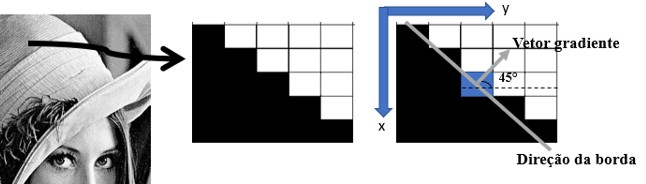
\includegraphics[width=.5\textwidth]{img/1-gradiente.jpg}
	\caption{Vetor gradiente representado sobre a imagem}
	\label{img:exemplo1}
\end{figure}

\begin{equation}
\alpha (x,y) = \arctan(\frac{Gx}{Gy}) 
\label{eq:angulo}
\end{equation}

\begin{equation}
M(x,y) = \sqrt{(Gx)^2 + (Gy)^2} 
\label{eq:modulo}
\end{equation}

O gradiente é uma importante ferramenta para encontrar as borda, entretanto, como aplicar a derivada em um sistema com valores digitais? Para isso se utiliza uma aproximação da derivada parcial, que é aplicada pixel-a-pixel. Como já visto, a deriva é conceituada como a variação instantânea de uma dada função, generalizando esse conceito pode-se chegar as equações \ref{eq:gradientex} e \ref{eq:gradientey}, representada matricialmente pela imagem(a) \ref{img:mascara}. Isso significa que a diferenciação em um elemento da imagem pode ser vista como a diferença das intensidades dos elementos vizinhos.  

\begin{equation}
	Gx = \frac{\partial f(x,y)}{\partial x} = f(x + 1,y) - f(x,y)
	\label{eq:gradientex}	
\end{equation}

\begin{equation}
	Gy = \frac{\partial f(x,y)}{\partial y} = f(x ,y+ 1) - f(x,y)
\label{eq:gradientey}
\end{equation}

É importante salientar que essa forma de calcular o gradiente não é suficiente quando se trata de bordas diagonais, uma vez que a intensidade de cor dos pixeis vizinhos na diagonal não são considerados. Uma forma de solucionar esse problema é construir uma mascara de 2 dimensões que detecte variações de todos os 8 vizinhos. Segundo \cite{ProcDigital} essas mascaras recebe o nome de \textit{Operadores de Prewitt} e pode ser vista na imagem(b) \ref{img:mascara}. O método de Canny utiliza o \textit{Operador de Sobel}, o qual valoriza os pixel mais próximos por meio de um peso com valor 2, representado pela imagem(c) \ref{img:mascara}. Para exemplificar a aplicação do operador Sobel, o aplicaremos sobre a imagem(a) \ref{img:gradiente}, uma figura constituída apenas por duas tonalidades de cinza, 0 e 255. Como só há duas cores, a variação só é detectada exatamente quando há a troca de cores, como pode ser visto na imagem(c) \ref{img:gradiente}, que representa o gradiente na direção y, de tal forma que a variação é vista como uma linha branca traçada próximo do centro. Como não há variação de cor quando se analisa o eixo x a "deriva" é igual a zero, logo a imagem do gradiente em x (figura (b) \ref{img:gradiente}) (Gx) é constituída de zeros, logo representada apenas por preto.

\begin{figure}[h!]
	\centering
	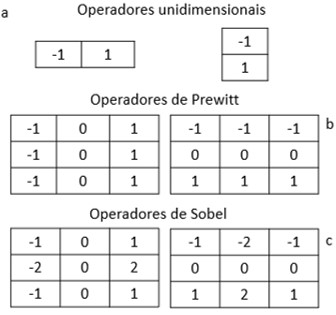
\includegraphics[width=.5\textwidth]{img/mascara.jpg}
	\caption{Matrizes representantes dos operadores diferenciais}
	\label{img:mascara}
\end{figure}

\begin{figure}[h!]
	\centering
	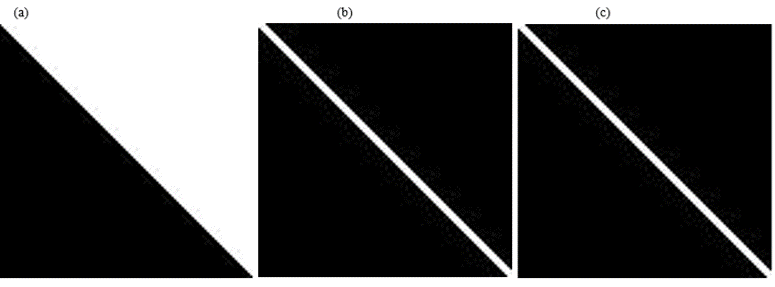
\includegraphics[width=.5\textwidth]{img/gradiente.png}
	\caption{Representação da aplicação do gradiente na direção de x (b) e y (c)}
	\label{img:gradiente}
\end{figure}

Como forma de demonstrar o método de detecção da variações de cores, suponha que se deseja detectar a existência de uma borda no pixel destacado (na cor azul) da imagem \ref{img:exemplo1}. Suponha também que a cor escura seja igual a 0 e a cor clara seja 255. O primeiro passo é centralizar o pixel com o centro do operador, iremos utilizar o operador de Sobel, veja a imagem \ref{img:Primeira}.

\begin{figure}[h!]
	\centering
	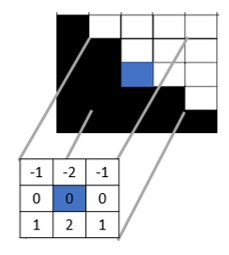
\includegraphics[width=.3\textwidth]{img/1im.jpg}
	\caption{Centralizando pixel com o operador}
	\label{img:Primeira}
\end{figure}

Multiplica-se assim o pixel analisado e seus 8 vizinhos pelo valor correspondente à sua posição no operador. Esse processo resultará uma matriz com as mesmas dimensões do operador. O próximo passo é fazer o somatório dos elementos desse array resultante, detectamos dessa forma a intensidade do gradiente em uma das direções. Por fim, o valor obtido é colocado, na mesma posição do pixel que foi estudado, em uma nova matriz, denominada como matriz de gradientes. Observe esses processos na imagem \ref{img:grady}. 

\begin{figure}[h!]
	\centering
	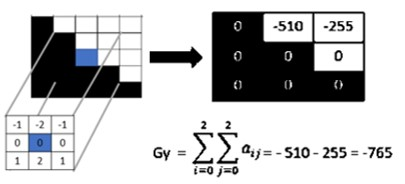
\includegraphics[width=.3\textwidth]{img/grady.jpg}
	\caption{Encontrando a intensidade do gradiente}
	\label{img:grady}
\end{figure}

Realizando os mesmos procedimento com o operador em x, detectamos que $Gx = 765$. Utilizando as operações da equação \ref{eq:angulo} constatamos que $\alpha = -45°$ o que equivale a 135° considerando o quadrante positivo. Por fim, usando a equação \ref{eq:modulo} é possível deduzir uma valor representante da variação nas duas dimensões. Realizando as contas obtemos que $M = 765*\sqrt{2}$. Esse valor é alocado em uma nova matriz, na posição correspondente ao pixel estudado.


   

\subsection{Supressão do não máximo}
\subsection{Limiarização}

O processo final da detecção de bordas elaborado por Canny, a limiarização, consiste em separar a imagem em duas partes onde uma representa a região de interesse, a borda, e a outra parte representa o fundo da imagem.  Esse processo se resume na identificação da diferença de cinza, através de um valor limiar, denominado binarização da imagem. [Morgan at. Al 2008]

Esse limiar traduz-se em limitar o máximo e mínimo das características de uma imagem, se tratando disso, os valores abaixo e acima desse limite são tratados de maneira diferentes, podendo ser interpretados como borda ou fundo. [Silva, 2000] 
Desse modo o processo de limiarização produz uma imagem bem definida, distinguindo o fundo e o objeto (área de interesse) através da diferença bem definida do nível de cinza da imagem, ou seja, a diferença de intensidade entre um pixel e outro é maior. Conforme Grando(2005) podemos definir a limiarização como: [Morgan at. Al 2008]
	     
\begin{equation}
 G(x,y)=\begin{cases} 1 & f(x,y)>T \\ 
   
 0 & f(x,y)\le T \end{cases}
\end{equation}
	     
Onde f(x,y) é a imagem de entrada, T é o valor de limiar e g(x, y) é a imagem de saída, imagem limiarizada [Morgan at. Al 2008]. Podemos observar que na fórmula os valores maiores que o limiar são considerados como borda, e os valores abaixo desse limiar são considerados como fundo. Assim, a imagem produzida, g(x, y), será uma imagem com o número de ruídos reduzidos.

\section{Desenvolvimento do algoritmo}

Como apresentado, o objetivo geral deste artigo é demonstrar de forma prática a aplicação do cálculo de derivadas na área da Engenharia de Computação. Com esse intuito, foram realizadas pesquisas e experimentações para aprofundar o conhecimento em processamento de imagens. Além disso, um dos objetivos específicos foi desenvolver um algoritmo capaz de encontrar as bordas de um objeto em uma imagem e com isso retornar dados da sua medição, demonstrando uma aplicação dos dados extraídos de uma imagem processada.

A detecção da variação de intensidade em imagens é algo canônico na visão computacional
\citep{canny1983variational}, e é baseado nos estudos do método aplicado por John Canny para detecção de bordas que foram realizadas as experimentações. Retomando o objetivo geral do trabalho, o entendimento do método Canny foi necessário, dado que este se baseia na aplicação da primeira derivada da função Gaussiana.

A primeira etapa foi dedicada a desenvolver um algoritmo que através da manipulação da matriz de uma imagem, retornasse uma matriz resultante apenas com elementos binários. Utilizando a biblioteca OpenCV, foi desenvolvido um algoritmo que recebe uma imagem e a salva na forma matricial, onde cada pixel representa um elemento da matriz. O número atribuído a esse pixel, ou seja, ao elemento dessa matriz, é um valor do sistema RGB. Na sequência, transformam-se os valores dos canais RGB em um único representante na escala de cinza. Essa modificação é necessária para diminuir as variações entre as cores dos pixels. Por fim, é aplicado o método Canny, que é capaz de identificar mudanças na intensidade dos pixels da imagem para detectar a presença de bordas.

\section{Resultados}

Retomando um dos objetivos específicos deste trabalho, utilizamos a matriz binária gerada após aplicação do método Canny para realizar a medição de um objeto contido na imagem. Interpretando a matriz resultante como um sistema de coordenadas, onde as colunas representam o eixo x e as linhas representam o eixo y, foram criadas duas funções:

- A primeira função, busca pelo primeiro e pelo último elemento (x, y) da matriz cujo valor seja 1, ou seja, presença de borda. Subtraindo o componente y do ultimo elemento, pelo componente y do primeiro elemento, obtêm-se a altura em pixels do objeto. Essa função limita-se a medir objetos sem que haja aplicação de rotações.

- A segunda função, faz uma varredura na matriz em sentidos opostos, encontrando duas quinas no objeto. Dessa maneira, com a informação da coordenada (x, y) das quinas, utilizou-se o conceito de distância entre dois pontos para encontrar o valor em pixels de uma quina à outra. Essa função limita-se a medir objetos com quinas bem definidas, quando a medida é o diâmetro, por exemplo, utiliza-se o método citado anteriormente. Rotações que não envolvam o eixo de profundidade são medidas sem que haja danos ao resultado. 

\begin{figure}[h!]
	\centering
	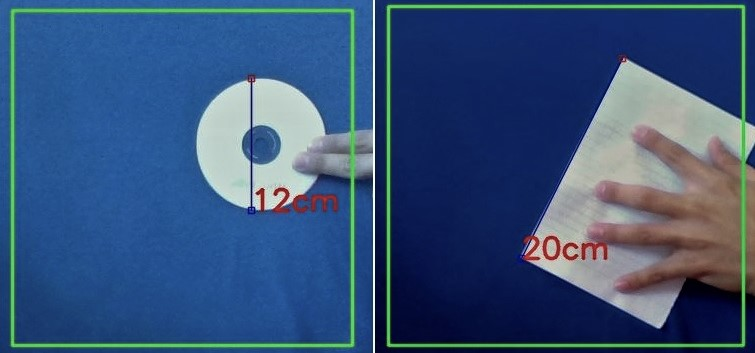
\includegraphics[width=.3\textwidth]{img/01-IMAGEM1.jpg}
	\caption{Demonstração dos métodos de medição}
	\label{img:img1}
\end{figure}

Foram realizadas diversas experimentações para constatar a correlação entre a medida em pixels, e a medida real do objeto em milímetros. Neste processo controlaram-se algumas variáveis, como: a distância do objeto à câmera; a rotação do objeto; e o processo de limiarização do método Canny.

\begin{figure}[h!]
	\centering
	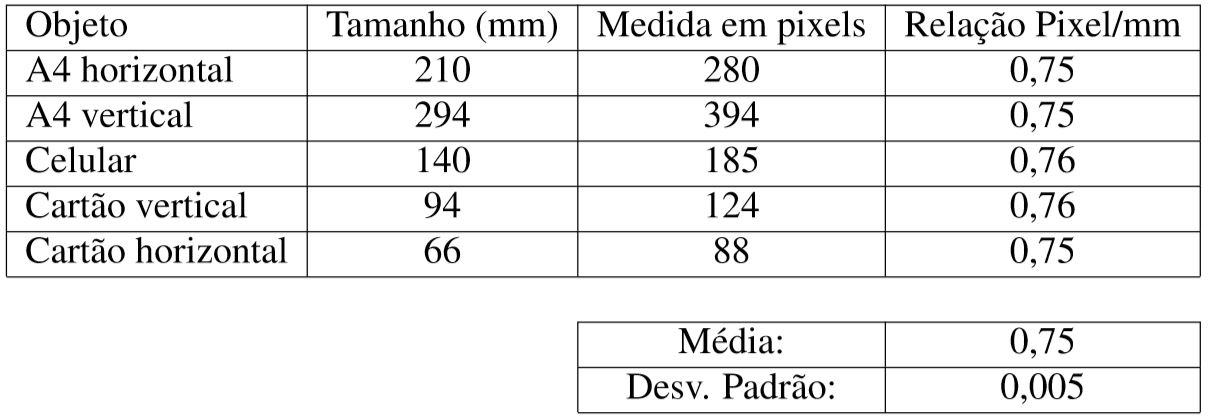
\includegraphics[width=.3\textwidth]{img/02-TABELA1.JPG}
	\caption{Resultados das medições realizadas a 500mm de distância}
	\label{img:tabela1}
\end{figure}

\begin{figure}[h!]
	\centering
	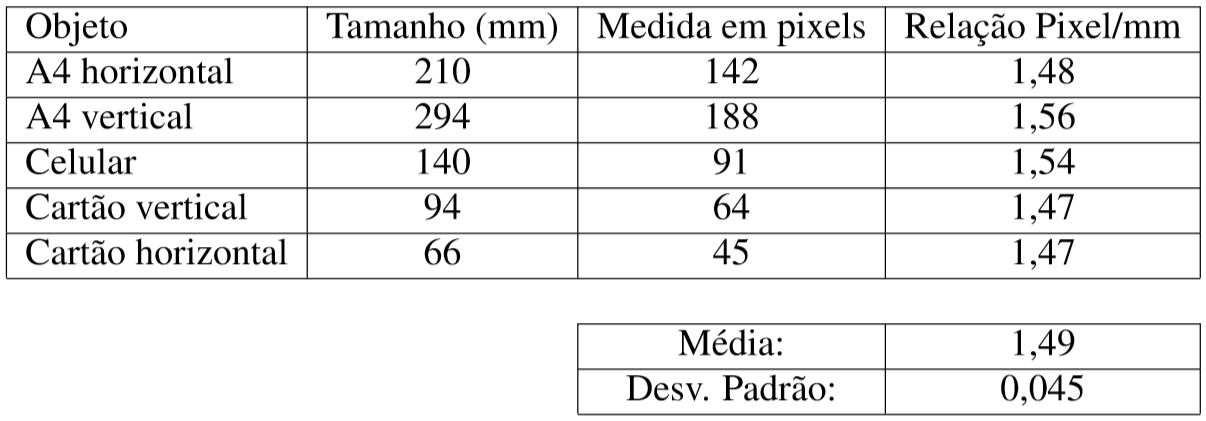
\includegraphics[width=.3\textwidth]{img/03-TABELA2.JPG}
	\caption{Resultados das medições realizadas a 1000mm de distância}
	\label{img:tabela2}
\end{figure}

Como pode ser observado na figura \ref{img:tabela1}, o desvio padrão da relação pixel/milímetros é bem inferior àquela constatada na figura \ref{img:tabela2}. Isso indica que quanto menor a distância entre a câmera e o objeto medido, maior será a repetitividade do processo, assim como melhor será a precisão. Isso está relacionado com a perda de detalhes do objeto ao afastá-lo da câmera. 

Buscando realizar medições em tempo real, foi necessário criar uma etapa para estabelecer uma relação inicial entre pixels e centímetros a ser mantida durante a medição de novos objetos. Este processo consiste na utilização de um objeto com dimensões conhecidas, e a partir da medição deste objeto, dada em pixels, computar a relação entre pixel e centímetro a ser mantida.

\begin{figure}[h!]
	\centering
	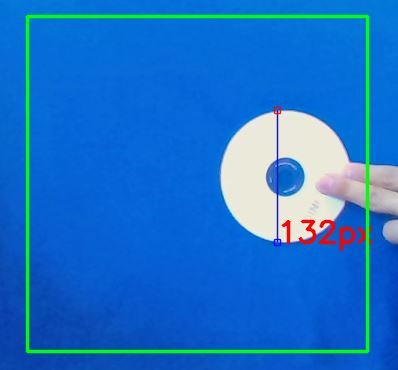
\includegraphics[width=.3\textwidth]{img/04-IMAGEM2.JPG}
	\caption{Computando a altura em pixeis para ser utilizado como referência}
	\label{img:img2}
\end{figure}

A imagem \ref{img:img2}, o diâmetro do CD foi equivalente à 132 pixels. Como um CD padrão tem diâmetro de 12,0 centímetros, o software computou a relação pixel/centímetro equivalente à aproximadamente 0,091 centímetros por pixel. Esta relação foi estabelecida com a câmera a uma distância de 750 milímetros do objeto, e, portanto, mantida para as demais medições.

Como as bordas que não representam o objeto, e as bordas do objeto são armazenadas da mesma maneira, ao analisar a imagem completa, a presença de detalhes indesejados impedia o processo de medição. Essa situação era devido ao fato de o algoritmo procurar o primeiro e o último elemento da matriz que representasse borda, e ao encontrar falsas bordas, ou bordas que não representam o objeto, falhas eram geradas. Percebido isso, foi desenvolvida uma nova função no programa com a função de delimitar a região de interesse. Esta função tem como objetivo reduzir a área de busca por bordas, transformando a matriz da imagem em uma matriz menor.

\begin{figure}[h!]
	\centering
	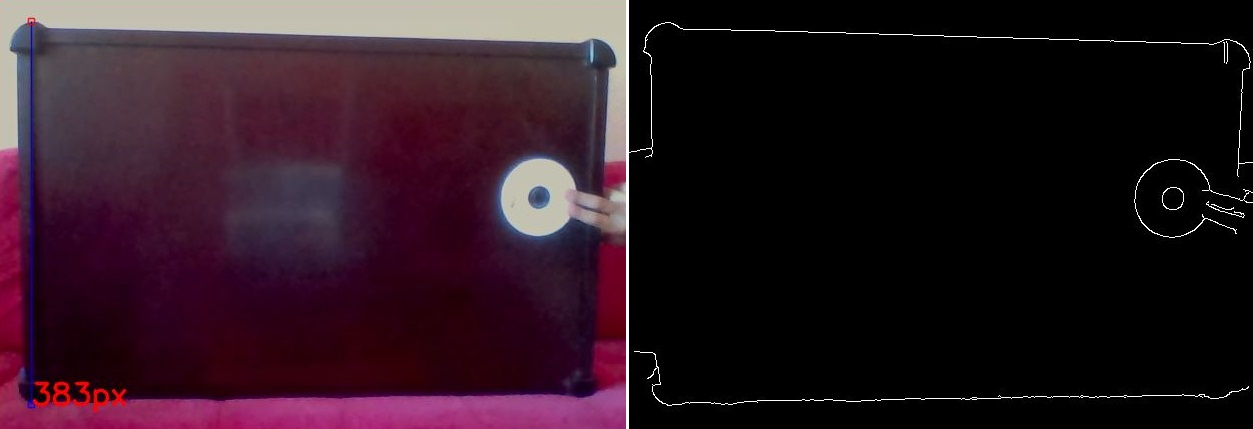
\includegraphics[width=.5\textwidth]{img/05-IMAGEM3.jpg}
	\caption{Detecção de borda sem a região de interesse}
	\label{img:img3}
\end{figure}

\begin{figure}[h!]
	\centering
	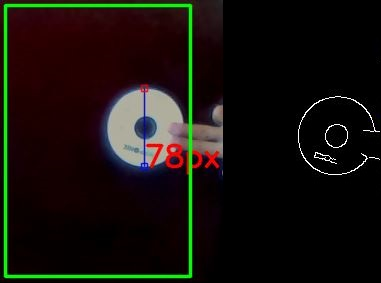
\includegraphics[width=.3\textwidth]{img/06-IMAGEM4.jpg}
	\caption{Detecção de borda dentro da região de interesse}
	\label{img:img4}
\end{figure}

Como pode ser observado na figura \ref{img:img3}, em que não há delimitação da área de busca, o algoritmo retornou uma altura em pixels equivalente à 383px. Já na imagem \ref{img:img4}, a região de busca por bordas corresponde à área interna do retângulo de contorno verde, isso significa que somente o que estiver compreendido na região de interesse será analisado.

Além do problema com a região de interesse, houve também a necessidade de permitir que o usuário pudesse modificar, quando necessário, a limiarização desejada para o processo. Pois, a aplicação da limiarização é difícil e envolve experimentação. “A permanência de falsas bordas, após a limiarização, pode ter como motivo a escolha de um limiar baixo, ou alto demais” (Do Vale and DAL POZ 2002,p. 9). Na imagem \ref{img:img4} as bordas ficam restritas ao objeto, já na figura \ref{img:img5}, ocorre a presença de falsas bordas, sendo possível perceber o impacto de uma limiarização mal aplicada, o que interfere na medição.

\begin{figure}[h!]
	\centering
	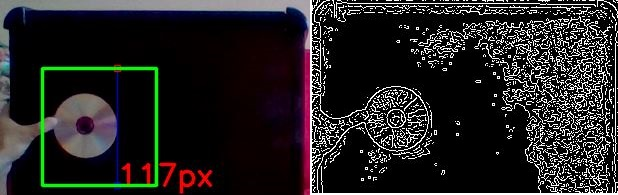
\includegraphics[width=.5\textwidth]{img/07-IMAGEM5.jpg}
	\caption{Detecção de borda com limiarização mal aplicada}
	\label{img:img5}
\end{figure}

Por fim, reduzindo a região de interesse, e permitindo a limiarização durante o processo de medição, o algoritmo foi capaz de retornar medições dos objetos com uma precisão de 0,0962 centímetro, ou seja, inferior à 1 milímetro (vide Figura \ref{img:tabela3}). Esse é um resultado aceitável, visto que se buscava a demonstração de uma utilização dos dados de saída do método de detecção de borda. Porém, o fato de trabalharmos com uma câmera 2D, implicou na perda de percepção de profundidade. Logo, quando há rotação do objeto em profundidade a medição passa a se invalidar. Aprofundar os cálculos para encontrar medições do objeto independente da rotação, é uma das possíveis vertentes que este trabalho poderá seguir, portanto não será abordada essa variável de processo.

\begin{figure}[h!]
	\centering
	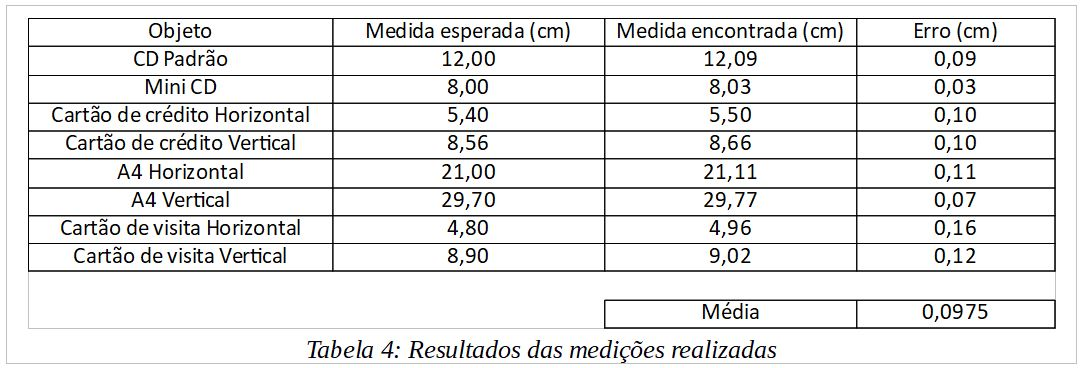
\includegraphics[width=.5\textwidth]{img/T4.JPG}
	\caption{Resultados de medições}
	\label{img:tabela3}
\end{figure}

\bibliography{references} 

\end{document}
